\chapter{Épidémiologie de la Chikungunya}


\section*{Introduction}
Le chikungunya est une maladie virale transmise à l'homme par des moustiques infectés par le virus du chikungunya. Les moustiques impliqués dans la transmission sont Aedes aegypti et Aedes albopictus~\cite{intro}. 
\section{Origine de la Chikungunya}
La fièvre \textbf{Chikungunya} est une maladie virale décrite pour la première fois en 1952 lors d'une épidémie dans le sud de la \textbf{Tanzanie}. Le nom vient d'un mot de la langue \textit{Makonde}, parlée dans le sud-est de la Tanzanie et le nord du Mozambique, qui signifie "\textit{devenir contorsionné}" ou "\textit{ce qui se plie}". Le virus a été isolé pour la première fois en Thaïlande en 1958.\cite{origin}

\section*{Évolution géographique et épidémiologique}
En \textbf{avril 2005}, il a été confirmé que le CHIKV était à l'origine d'une épidémie de maladie ressemblant à la dengue sur les îles Comores, situées au large de la côte est du Mozambique septentrional ; il s'agissait de la première émergence connue du CHIKV dans la région du sud-ouest de l'océan Indien. En raison de similitudes cliniques, cette épidémie a d'abord été suspectée d'être causée par le virus de la dengue, soulignant le fait que la maladie CHIKV est souvent mal diagnostiquée et que le nombre réel de cas dans une région donnée peut être sous-estimé. Peu après, les premiers cas de CHIKV ont été signalés à Mayotte, à Maurice et sur l'île française de La Réunion. Le nombre de cas dans ces régions a rapidement augmenté, notamment en raison de taux d'attaque atteignant \textbf{35\%} à \textbf{75\%}. À la fin de l'année \textbf{2005}, après une période apparente d'environ 32 ans pendant laquelle le CHIKV n'a pas été détecté, l'Inde a signalé des cas de maladie à CHIKV dans de nombreux États, le nombre officiel de cas suspects atteignant finalement plus de 1,3 million. L'épidémie de CHIKV a continué à se propager, provoquant d'importantes flambées au Sri Lanka et dans de nombreux autres pays d'Asie du Sud-Est. Au cours de cette épidémie, le CHIKV a été introduit dans des pays où il n'est pas endémique par des voyageurs virémiques, et la transmission autochtone du CHIKV a été observée pour la première fois dans de nombreux pays, dont l'Italie, la France, la Nouvelle-Calédonie, la Papouasie-Nouvelle-Guinée, le Bhoutan et le Yémen. La propagation rapide et explosive du CHIKV a incité l'Organisation panaméricaine de la santé (OPS) et les Centers for Disease Control and Prevention (CDC) à publier un guide de préparation qui prévoyait de futures épidémies potentielles de CHIKV dans les Amériques. Cette prédiction s'est maintenant concrétisée, puisqu'en décembre 2013, l'Organisation mondiale de la santé (OMS) a signalé la première transmission locale du CHIKV dans l'hémisphère occidental, sur l'île caribéenne de Saint-Martin. Le 18 juillet 2014, le CHIKV avait provoqué plus de 440 000 cas de maladie dans plus de 20 pays des Caraïbes, d'Amérique centrale et d'Amérique du Sud (Fig. 1). En outre, les CDC ont signalé plus de 230 cas importés d'infection à CHIKV sur le territoire continental des États-Unis, ainsi que des cas acquis localement en Floride. Ainsi, en moins de 10 ans, le CHIKV s'est propagé depuis les côtes du Kenya dans l'océan Indien, le Pacifique et les Caraïbes, provoquant des millions de cas de maladie dans plus de 50 pays. En d'autres termes, le CHIKV est redevenu un véritable agent pathogène mondial.
\begin{figure}[!h]
	\begin{center}
		%taille de l'image en largeur
		%remplacer "width" par "height" pour régler la hauteur
		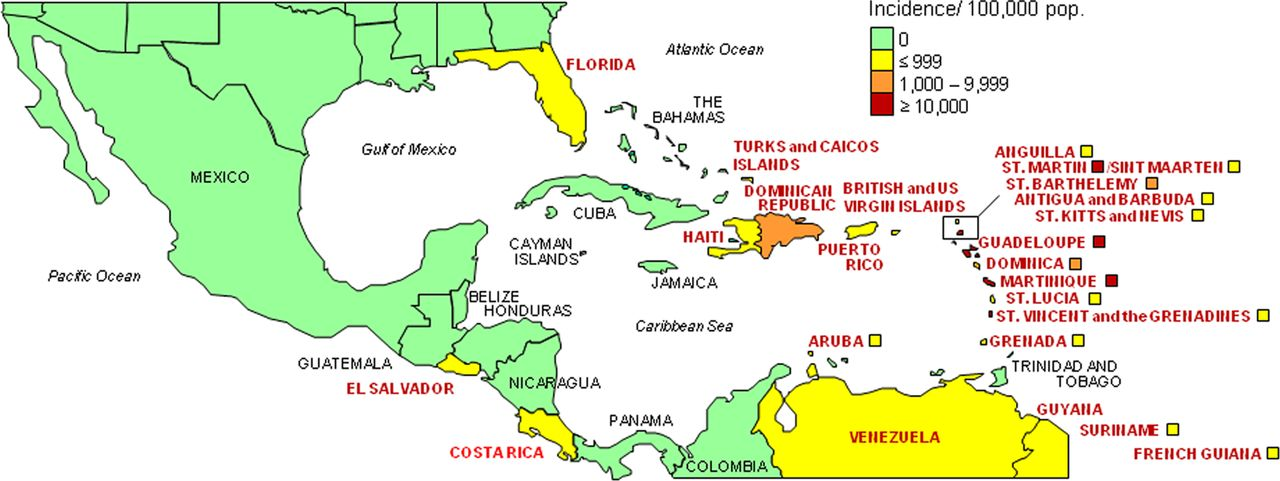
\includegraphics[width=10cm]{images/zjv9990995820001}
	\end{center}
	%légende de l'image
	\caption{CHIKV in the Western Hemisphere.}
	\label{fig:chikvwestern}
\end{figure}

\section{Agent Pathogène}
Le virus du chikungunya (CHIKV), un alphavirus transmis par les moustiques, dont le génome est constitué d'un ARN monocaténaire à sens positif de ∼12 kb~\cite{JournalofVirology}.
\begin{figure}[!h]
	\begin{center}
		%taille de l'image en largeur
		%remplacer "width" par "height" pour régler la hauteur
		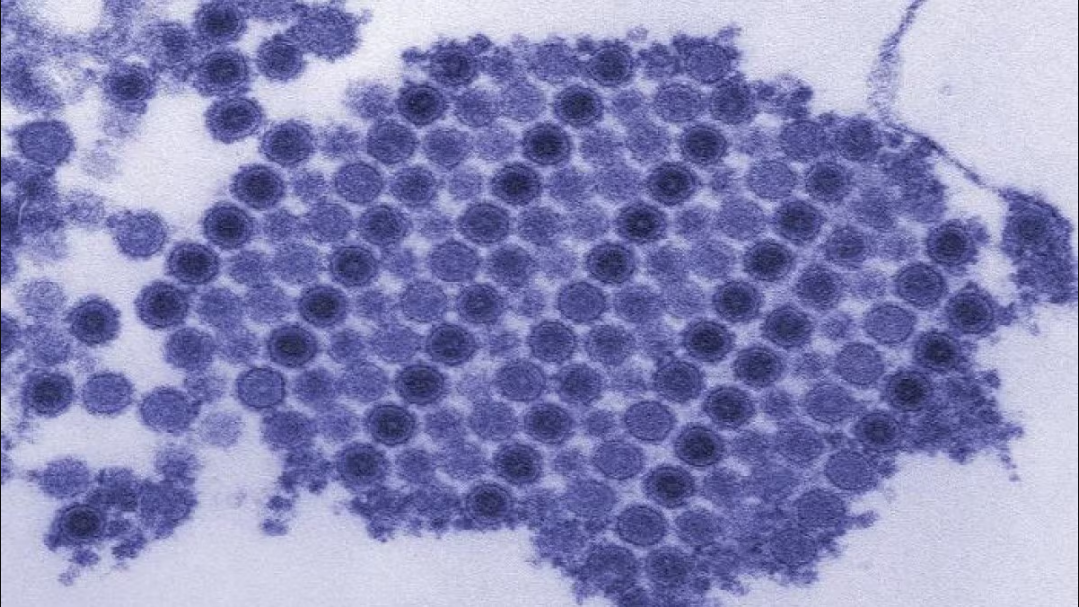
\includegraphics[width=10cm]{images/CHIK_17550_TEM}
	\end{center}
	%légende de l'image
	\caption{Electron microscopic image of chikungunya virus}
	\label{fig:chikv} 
\end{figure}

\section{Mode de Transmission}
Comprendre les mécanismes de transmission du virus chikungunya est essentiel pour développer des stratégies de prévention efficaces. Cette section examine les principaux vecteurs de la maladie, les conditions environnementales qui favorisent la propagation du virus et les dynamiques de transmission entre les hôtes humains et animaux.
\subsection{Vecteurs : Les moustiques Aedes}
Le virus du chikungunya est un alphavirus, similaire aux virus de Mayaro et de Ross River, appartenant à la famille \textit{Togaviridae}, au genre \textit{Alphavirus}. Le virus du chikungunya est principalement transmis à l'homme par la piqûre d'un moustique infecté, principalement \textit{Aedes aegypti} (Voir Figure \ref{fig:aedes}) et \textit{Ae. albopictus} .
\begin{figure}[!h]
	\begin{center}
		%taille de l'image en largeur
		%remplacer "width" par "height" pour régler la hauteur
		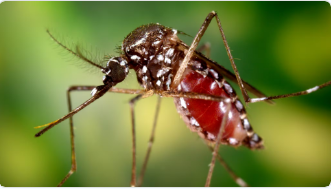
\includegraphics[width=7cm]{images/moustique}
	\end{center}
	%légende de l'image
	\caption{Aedes aegypti mosquito full of blood}
	\label{fig:aedes}
\end{figure} 

\subsection{La transmission}
Le \textbf{CHIKV} se transmet selon deux cycles différents :
\begin{itemize}
	\item \textbf{Cycle urbain} : transmission de l'homme au moustique.
	\item \textbf{Cycle sylvatique} : transmission de l'animal au moustique, puis à l'homme \cite{ganesan2017chikungunya}.
\end{itemize}
Le cycle sylvatique est la principale forme de transmission en Afrique \cite{ganesan2017chikungunya}. Ailleurs, dans les zones plus densément peuplées, le CHIKV se maintient principalement dans un cycle urbain, dans lequel les humains sont les principaux hôtes et les moustiques du genre \textit{Aedes} les vecteurs \cite{ganesan2017chikungunya} (voir figure\ref{fig:chikvtransmission}).
bien que \textit{Ae. aegypti} continue d'être un vecteur viral important, comme on l'a vu lors de la flambée épidémique dans les Caraïbes en 2013 \cite{ganesan2017chikungunya}.
La transmission verticale de la mère à l'enfant a été postulée pour expliquer les incidences postérieures à 2005 \cite{ganesan2017chikungunya}, étant particulièrement délétère lorsque :
\begin{itemize}
	\item la mère est infectée jusqu'à quatre jours après l'accouchement \cite{ganesan2017chikungunya},
\end{itemize}
bien que cette hypothèse ait été contestée \cite{ganesan2017chikungunya}.

 
\begin{figure}[!h]
	\begin{center}
		%taille de l'image en largeur
		%remplacer "width" par "height" pour régler la hauteur
		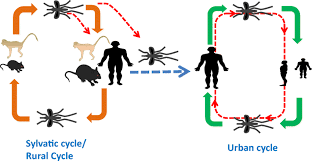
\includegraphics[height=5cm]{images/trans}
	\end{center}
	%légende de l'image
	\caption{Transmission mode Chikungunya}
	\label{fig:chikvtransmission}
\end{figure}
\newpage
\section{Symptômes et Diagnostic}
La reconnaissance des symptômes et l'établissement d'un diagnostic précis sont essentiels pour la gestion efficace des cas de chikungunya. Cette section examine les manifestations cliniques typiques de l'infection par le virus chikungunya ainsi que les méthodes diagnostiques utilisées pour identifier la maladie.
\subsection{Symptômes}
Chez les patients symptomatiques, la maladie à \textbf{CHIKV} se déclare généralement 4 à 8 jours (entre 2 et 12 jours) après la piqûre d'un moustique infecté. Elle se caractérise par une brusque poussée de fièvre, souvent accompagnée de fortes douleurs articulaires. Les douleurs articulaires sont souvent invalidantes et durent généralement quelques jours, mais peuvent être prolongées et durer des semaines, des mois, voire des années. D'autres signes et symptômes courants sont le gonflement des articulations, les douleurs musculaires, les maux de tête, les nausées, la fatigue et les éruptions cutanées. Comme ces symptômes se confondent avec ceux d'autres infections, notamment celles dues aux virus de la dengue et du Zika, les cas peuvent être mal diagnostiqués. En l'absence de douleurs articulaires importantes, les symptômes des personnes infectées sont généralement légers et l'infection peut passer inaperçue.

La plupart des patients se rétablissent complètement de l'infection ; toutefois, des cas occasionnels de complications oculaires, cardiaques et neurologiques ont été signalés dans le cadre d'infections par le \textbf{CHIKV}. Les patients situés aux extrémités du spectre d'âge sont plus exposés à une maladie grave. Les nouveau-nés infectés pendant l'accouchement et les personnes âgées souffrant de pathologies sous-jacentes peuvent devenir gravement malades et l'infection par le \textbf{CHIKV} peut augmenter le risque de décès~\cite{who2}.

Une fois qu'une personne est guérie, les données disponibles suggèrent qu'elle est probablement immunisée contre les infections futures~\cite{auerswald2018broad}.

\subsection{Méthodes de diagnostic}
Le diagnostic peut être retardé en raison de la confusion possible des symptômes avec ceux de la dengue ou du Zika. Les tests \textbf{\textit{immuno-enzymatiques}} (ELISA) peuvent être utilisés pour confirmer la présence d'anticorps \textbf{anti-CHIKV}, les niveaux d'anticorps IgM étant les plus élevés trois à cinq semaines après l'infection et persistant jusqu'à deux mois. La PCR peut également être utilisée pour génotyper le virus~\cite{JournalofVirology}.

\section{Méthodes de Contrôle et Traitement}

La gestion efficace de l'épidémie de chikungunya repose sur une combinaison de stratégies de contrôle des vecteurs et d'interventions médicales. Cette section explore les diverses approches utilisées pour prévenir la transmission du virus et traiter les symptômes chez les patients infectés.

\subsection{Méthodes de contrôle}
La prévention de l'infection en évitant les piqûres de moustiques est la \textbf{meilleure protection}. Les patients suspectés d'être infectés par le \textbf{CHIKV} doivent éviter les piqûres de moustiques pendant la première semaine de la maladie afin d'empêcher la transmission aux moustiques, qui peuvent à leur tour infecter d'autres personnes. 

La principale méthode pour réduire la transmission du \textbf{CHIKV} consiste à contrôler les moustiques vecteurs. Pour ce faire, il faut mobiliser les communautés, qui jouent un rôle essentiel dans la réduction des sites de reproduction des moustiques en :

\begin{itemize}
	\item vidant et en nettoyant chaque semaine les récipients contenant de l'eau,
	\item éliminant les déchets,
	\item soutenant les programmes locaux de lutte contre les moustiques.
\end{itemize}

Pendant les épidémies, des insecticides peuvent être :

\begin{itemize}
	\item pulvérisés pour tuer les moustiques adultes volants,
	\item appliqués sur les surfaces à l'intérieur et autour des conteneurs où les moustiques se posent,
	\item utilisés pour traiter l'eau dans les conteneurs afin de tuer les larves immatures.
\end{itemize}

Les autorités sanitaires peuvent également prendre des mesures d'urgence pour contrôler la population de moustiques.

Pour se protéger pendant les épidémies de \textbf{chikungunya}, il est conseillé de :

\begin{itemize}
	\item porter des vêtements qui minimisent l'exposition de la peau aux vecteurs qui piquent pendant la journée,
	\item utiliser des moustiquaires aux fenêtres et aux portes pour empêcher les moustiques de pénétrer dans les maisons,
	\item appliquer des répulsifs sur la peau exposée ou sur les vêtements en respectant scrupuleusement les instructions figurant sur l'étiquette du produit.
\end{itemize}

Les répulsifs doivent contenir du \textbf{DEET}, de l'\textbf{IR3535} ou de l'\textbf{icaridine}~\cite{WHO}.

\subsection{Options de traitement}
Le traitement actuel vise à atténuer la gravité des symptômes plutôt qu'à guérir la maladie. Le traitement repose principalement sur l'utilisation d'\textbf{antipyrétiques} et d'\textbf{AINS}. Cependant, aucune étude n'a évalué systématiquement l'efficacité de ces traitements, et les symptômes peuvent disparaître sans intervention. L'utilisation de \textbf{corticostéroïdes} pour le traitement de la phase aiguë a connu un succès mitigé et est utilisée avec hésitation en raison de la possibilité d'aggravation des symptômes après le traitement. Il est particulièrement important de maintenir des niveaux de liquide adéquats. 

Il existe également des preuves émergentes que les médicaments qui entravent le transport du cholestérol, tels que les composés \textbf{amphiphiles cationiques de classe II U18666A} et l'\textbf{imipramine}, peuvent être efficaces contre la fusion membranaire du \textbf{CHIKV}, et ont un potentiel d'action contre d'autres arbovirus.

Pour les arthralgies chroniques graves, des \textbf{antirhumatismaux modificateurs de la maladie (ARMM)}, notamment le \textbf{méthotrexate}, l'\textbf{hydroxychloroquine} ou la \textbf{sulfasalazine}, ont été proposés. Comme pour les traitements aigus, l'efficacité systématique des \textbf{DMARD} pour le traitement chronique est inconnue, bien que des rapports décrivent des résultats positifs avec une cessation des symptômes dans les 4 à 6 mois \cite{ganesan2017chikungunya}.

\section{Cas du Tchad}

L'analyse spécifique des cas de chikungunya au Tchad permet de comprendre l'impact de cette maladie dans un contexte régional spécifique. Cette section examine les caractéristiques épidémiologiques, les stratégies de contrôle et les défis rencontrés dans la gestion de l'infection par le virus chikungunya dans ce pays d'Afrique centrale.

\subsection{Point saillants}
\begin{figure}[!h]
	\begin{center}
		%taille de l'image en largeur
		%remplacer "width" par "height" pour régler la hauteur
		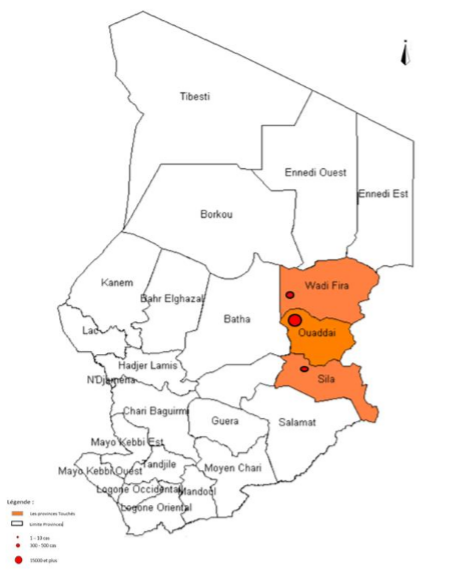
\includegraphics[height=8cm]{images/chadmap}
	\end{center}
	%légende de l'image
	\caption{Region infecté au Tchad}
	\label{fig:chikvintchadmap}
\end{figure}

\subsection{Contexte}

\begin{figure}[!h]
	\begin{center}
		%taille de l'image en largeur
		%remplacer "width" par "height" pour régler la hauteur
		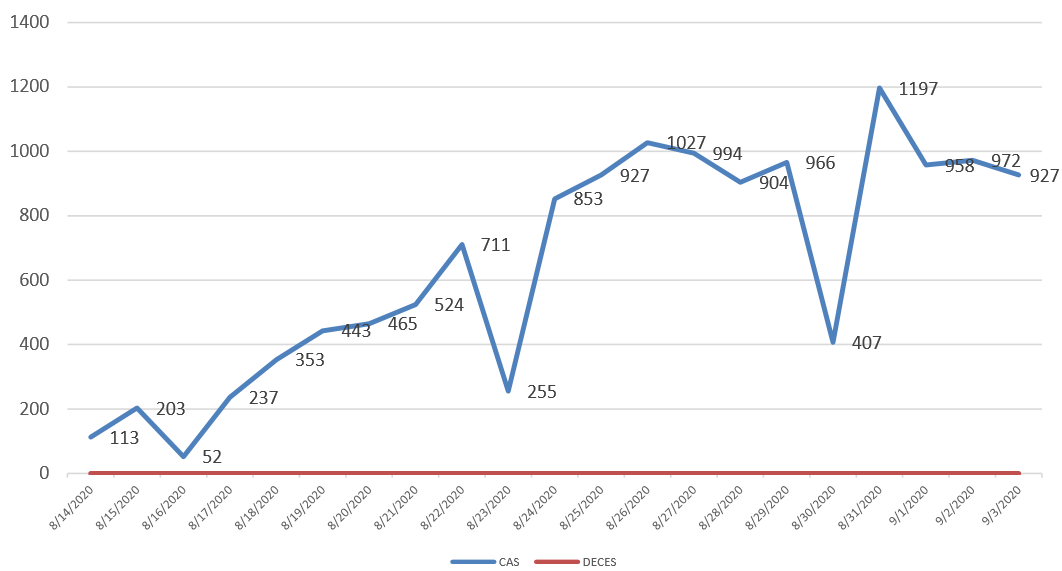
\includegraphics[width=10cm]{images/statsCaseChad}
	\end{center}
	%légende de l'image
	\caption{ Evolution journalière des cas et décès du Chikungunya}
	\label{fig:chikvevolution}
\end{figure}